\section{INTRODUCTION}

\justifying

This document is a guide for writing articles to be submitted to the \emph{Revista Ciencia en Desarrollo}. The author can rename this file and replace its content with that of the article. This template explains how to format the different components that can be inserted into the text (tables, graphs, equations, and references).

This step-by-step guide provides a detailed approach to writing a research-derived article presented at the international meeting of the Faculty of Sciences. Additionally, it offers a LaTeX template that conforms to the presentation guidelines required by the \emph{Revista Ciencia en Desarrollo}.

For this special issue, the \emph{Revista Ciencia en Desarrollo} will give priority to articles written in English. It is important to emphasize that all articles submitted for consideration must be unpublished, meaning they should not have been published in any other medium, whether in electronic or printed format, and should not have been submitted for evaluation by another journal.

Manuscript submitted to the journal must follow a standard structure that includes the following sections: introduction, materials and methods (methodology), results, conclusion, acknowledgments, and references.

The Introduction section plays a crucial role in providing a synthesized overview of the article's objective and the existing research context on the topic. In this part, background information should be presented clearly, the research problem should be articulated, and relevant previous works should be referenced. Additionally, the proposed approach or solution should be outlined, and the article's objectives should be established. It's worth noting that the introduction should be accessible to colleagues from various scientific disciplines and should not contain results or conclusions.


\section{METHODOLOGY}

\emph{The materials used in the project and the methods employed can be listed. If not applicable, this section can be omitted.}

This section explains how the research was conducted. However, only genuinely novel procedures should be described in detail.

Avoid the use of ambiguous terms such as 'frequently,' 'regularly,' and 'periodically.' Do not specify brand names of products or specific equipment models. It should be written in the past tense and in the third person, for example: 'was conducted,' 'was measured,' 'was mixed,' etc."

\section{RESULTS}

\emph{This section is the more important of the article.}

\emph{Figures and tables should contain enough information to be self-explanatory. Well-chosen scales, appropriately sized axis labels, clear symbols, and easily distinguishable data groups are necessary
}

The results should express what was obtained from the experiments or tests described in the materials and methods section. They are presented in a logical sequence in the text, using tables and figures. The repeated presentation of the same data in different forms should be avoided (the presentation of equations, figures, and tables is explained at the end of this document). The results and discussion should be explained and described in the past tense.





\section*{Equations}

Equations should be consecutively numbered in normal parentheses, in the right margin, without referencing the section where they are located; in other words, there should be independent numbering for equations. To write the equation, use the equation editor. It is important that symbols are defined before or immediately after the equation.

Units - there should always be a space after all units (except for temperature and percentages) and they should be in plain text format (not italicized or bold).
Example:

\begin{equation}
V(t) = V_{1}*e^{-\infty t } - \sum_{k-1}^{100}M_{k}*e^{-t}
\end{equation}

\section*{Figures and tables}


Tables are floaters, so their reference within the text should not depend on their location. However, whenever possible, tables should appear in the text following the section to which the table is referenced. They should be distributed throughout the text in a way that none appears after the References section.

All figures should be numbered consecutively according to their order of appearance, and, like equations, they should be referred to in the nearest text. They should be sharp, and photographs and figures should be original, in color, black and white, or grayscale, according to the author's preference, with a minimum resolution of 200dpi (dots per inch). The title should be written clearly to explain its content, located at the bottom, left-justified, in Times New Roman 10-point font, as shown in Fig.\ref{fig:Example_Fig}. In tables, the title will be presented at the top, with justified alignment, in Times New Roman 9-point font, as shown in Table \ref{fig:Example_Fig}.





\subsection{Tables} 

%
\begin{table}[!h]
    \label{tabla1}
	\caption{\small{Example
			$2\times 6$, with $m=10$ dates.}}
   \vspace{6pt}
	\centering {\small
		\begin{tabular}{ccrc}\hline
			$y_2$   &
			$\hat{y}_2$ &
			\multicolumn{1}{c}{$e_2$}   &
			$\hat{y}_2^*$\\ \hline
			52.1    & 54.2  &  $-2.76$      & 51.4  \\
			52.1    & 54.2  &  $ 1.10$      & 53.1  \\
			52.3    & 52.4  &  $-0.71$      & 51.7  \\
			59.9    & 59.3  &  $ 0.44$      & 59.7  \\
			59.9    & 59.3  &  $ 0.80$      & 60.1  \\
			51.7    & 54.0  &  $-1.33$      & 52.7  \\
			63.9    & 61.3  &  $ 0.27$      & 61.6  \\
			63.9    & 61.3  &  $ 1.31$      & 62.6  \\
			67.2    & 66.4  &  $-0.44$      & 66.0  \\
			64.8    & 61.0  &  $ 2.12$      & 63.1  \\ \hline
		\end{tabular}}
	\end{table}

If a  table is very large, it should be centered within a column (see table) \ref{Ejemplo_tabla2}).
	


\begin{table*}[htb]
	\centering\normalsize\caption{Table name}
  \vspace{6pt}
	\label{Ejemplo_tabla2}
	\begin{tabular}{cccccccc}\hline
		\multicolumn{8}{c}{Fluencia $(\varphi)$}\\
		\hline
		\multicolumn{2}{c}{$Y_0$} & \multicolumn{2}{c}{$A$} & \multicolumn{2}{c}{$B$} & \multicolumn{2}{c}{Statistics} \\
		\hline
		Value & Error & Value & Error & Value & Error & Chi-Cuadrado & Aj. R-Cuad. \\\hline
		8.75E-11&	5.56E-11&	3.89E-04&	-6.88E-06&	-0.48633&	0.00114&	5.43E-20&	0.99998\\\hline
		\multicolumn{8}{c}{Dosis (D)}\\
		\hline
		2.82E-11 & 1.76E-11 & 1.21E-04 & 1.81E-06 & -0.47602 & 9.59E-04 & 5.44E-21 & 0.99998 \\\hline
	\end{tabular}
\end{table*}



\subsection{Graphics}

They should be in postscript, pdf, png, etc. formats and should be saved in the same directory as the LaTeX file. The title should be at the bottom and centered, the digits on the vertical axis scale should be horizontal, and the text of the labels should be in the language of the article, as indicated in Figure \ref{fig:Example_Fig}.

Example:

\begin{figure}[H]
    \centering
    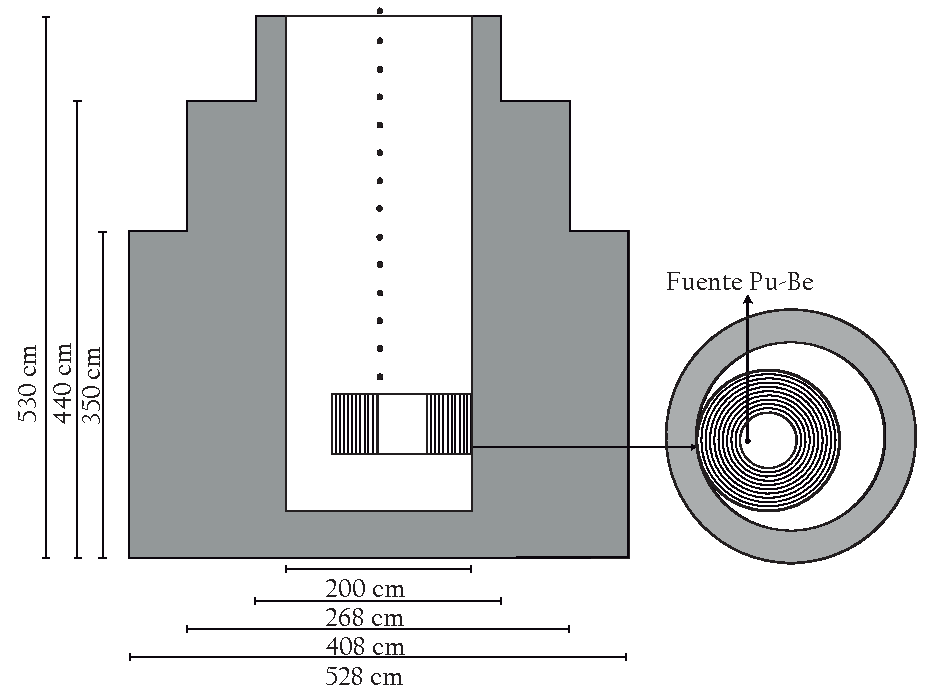
\includegraphics[scale=0.5]{Figuras/Art1Fig1.pdf}
    \caption{The caption should clearly explain the corresponding figure.}
    \label{fig:Example_Fig}
\end{figure}




\section{CONCLUSIONS.}

Conclusions should be clear and concise and can be enumerated. Their content should not substantially duplicate the abstract. They should express the final balance of the research or the application of knowledge on the topic. Discussion should revolve around the implications of the study and its relevance to the field of knowledge. It is suggested not to draw more conclusions than the results allow. This section typically mentions future work that can be carried out on the subject along with corresponding recommendations.

\noindent\footnotesize{{\bf Funding:} Please provide the funding entity here (if applicable).}\\

In addition to the acknowledgments, a conflict of interest declaration must be made.

\footnotesize{{\bf Declaration:} The authors declare no conflicts of interest.}



\section{ACKNOWLEDGEMENTS}

This section is necessary for research articles, where the author acknowledges individuals or institutions that assisted in their research. It may include grants and institutions that funded the research, commercial firms, official or private entities, professional associations, and collaborators. This section is optional for reflection articles. It is not a numbered section.

\textbf{Las referencias  se incluirán en el texto mediante números arábigos entre corchetes cuadrados  [ ], alineados con la escritura (formato IEEE), si son varias referencias juntas, se separarán con comas. Se enumerarán correlativamente
por orden de citación, apareciendo la lista al final del texto después de la sección de conclusiones o agradecimientos \cite{1},\cite{2}, \cite{3}.
}

\emph{
El estilo de referencias bibliográficas IEEE  es ampliamente utilizado en campos como la ingeniería, la electrónica y la informática. Aquí te presento cómo formatear las referencias bibliográficas en el estilo IEEE:}

\textbf{Libro:}

Apellido del autor, Inicial(es). (Año). Título del libro. Editor.

Ejemplo:

Smith, J. (2000). Introduction to Electrical Engineering. XYZ Publications.


\textbf{Capítulo de libro en una obra colectiva:}

Apellido del autor del capítulo, Inicial(es). (Año). "Título del capítulo". En Inicial(es) Apellido del editor (Ed.), Título del libro (páginas del capítulo). Editor.

Ejemplo:

Brown, R. (2015). "Advanced Circuits." En S. Johnson (Ed.), Electrical Engineering Handbook (pp. 112-135). ABC Publications.

\textbf{Artículo de revista:}

Apellido del autor, Inicial(es). (Año). "Título del artículo". Título de la revista, Volumen(Número), páginas.

Ejemplo:

Garcia, M. (2018). "An Analysis of Power Grids." IEEE Transactions on Power Systems, 30(2), 567-578.


\textbf{Conferencia o artículo de conferencia:}

Apellido del autor, Inicial(es). (Año, Mes de la conferencia). "Título del artículo". En Nombre de la conferencia (páginas). Editor.

Ejemplo:

Johnson, A. (2020, Julio). "Advancements in Robotics." En Proceedings of the International Robotics Conference (pp. 45-53). IEEE.

\textbf{
Documento en línea:}

Apellido del autor, Inicial(es). (Año). "Título del documento." Nombre del sitio web. [En línea]. Disponible en: URL. [Fecha de acceso: Día, Mes, Año].

Ejemplo:

Davis, S. (2019). "Introduction to Machine Learning." Machine Learning Central. [En línea]. Disponible en: https://www.example.com/ml-intro. [Fecha de acceso: 10 Septiembre 2023].

\textbf{Tesis:}

Apellido del autor, Inicial(es). (Año). "Título de la tesis." Tesis de Maestría/Doctorado, Nombre de la Universidad, Ciudad, País.

Ejemplo:

Chen, Q. (2017). "Design and Optimization of Communication Networks." Tesis de Doctorado, Universidad de California, Los Ángeles, EE. UU.
Recuerda que el formato exacto de las referencias puede variar según las directrices de la revista, conferencia o institución a la que envíes tu trabajo. Asegúrate de consultar las pautas específicas para garantizar que tus referencias cumplan con los requisitos del estilo IEEE que se solicitan.
